\documentclass[sigconf,review,anonymous]{acmart}
% WWW 2027 Research Track (long paper)
% 8 pages main + references (+ optional appendix) <= 12 total

\usepackage{booktabs}
\usepackage{placeins}
\usepackage{balance}
\usepackage{xcolor}
\emergencystretch=1.5em

\settopmatter{printacmref=true}
\renewcommand\footnotetextcopyrightpermission{\footnotetext{\hspace{-1.5em}}}

\newtheorem{proposition}{Proposition}
\newtheorem{definition}{Definition}

\acmConference[WWW '27]{Proceedings of the ACM Web Conference 2027}{April 2027}{}
\acmYear{2027}

\begin{document}

\title{SynthFlood: Ambient Synthetic Content Buys Web-Agent Decisions}

\author{Anonymous Author(s)}
\affiliation{\institution{Anonymous Institution}\city{}\country{}}

\begin{CCSXML}
<ccs2012>
   <concept>
       <concept_id>10002951.10003260.10003260</concept_id>
       <concept_desc>Information systems~World Wide Web</concept_desc>
       <concept_significance>500</concept_significance>
   </concept>
   <concept>
       <concept_id>10010147.10010178.10010179</concept_id>
       <concept_desc>Computing methodologies~Artificial intelligence</concept_desc>
       <concept_significance>300</concept_significance>
   </concept>
</ccs2012>
\end{CCSXML}

\ccsdesc[500]{Information systems~World Wide Web}
\ccsdesc[300]{Computing methodologies~Artificial intelligence}

\keywords{web agents, synthetic content, ambient contamination, dose--response, provenance, e-commerce}

\maketitle

\section{Introduction}
\label{sec:intro}
% numbers finalized from P1 v4 + P4A/E + P4C outputs (2026-10-10).

Web agents have crossed from demos to deployment: they shop, book, and
compare on our behalf, turning the Web's product pages from artifacts that
\emph{inform humans} into signals that \emph{direct machine decisions}. At
the same time, the supply side of those pages is being rewritten. An
estimated 27.5\% of tokens passing common quality filters on the open Web
are now AI-generated, and the share is climbing monthly \cite{russell2026much};
measurement studies document machine-generated catalogs flooding music
platforms \cite{wu2026empirical} and scientific publishing \cite{oh2026science}.
This content is not adversarial in the classical sense: much of it is produced
by ordinary commercial incentives --- search-optimized content farms,
counterfeit-style listing clones, review inflation --- and a whole research
program now studies how to \emph{optimize} content for generative engines
\cite{wu2025what,bagga2025egeo,nimase2026geobench} and how to detect the
result \cite{chu2026geoflag,zheng2026countergeobench,li2026when}. The
inevitable consequence is that agentic systems increasingly browse a Web
whose supply of plausible, keyword-rich, well-rated listings no longer
correlates with actually satisfying the user's goal.

This paper asks a question that, to our knowledge, no prior work has measured
in a controlled setting: \textbf{does ambient, non-targeted synthetic content
silently erode the decision quality of web agents?} Existing evaluations of
agents under Web pollution attack them deliberately: programmatic mini-internets
with adversarially curated falsehoods \cite{shah2026synthetic}, attacker-written
endorsement pages steering search agents \cite{chen2026much}, or prompt
injection and memory poisoning \cite{cao2026ward,yang2026zombie,syros2026muzzle}.
Upstream of the decision, retrieval-level studies show that cumulative AI
pollution degrades search quality \cite{yu2026retrieval}. But ambient
contamination is a different regime: no adversary knows the user's goal, so
no page is crafted to defeat a specific decision. The threat is statistical,
not surgical --- and whether it materially matters for agent \emph{economics}
(choice quality, wasted spend, calibrated confidence) is unknown.

Measuring this regime requires solving a confound that has kept prior work at
the retrieval layer: if we simply compare agent success before and after
contaminating a benchmark, any degradation could stem from task difficulty
rather than choice quality. We therefore build \textbf{SynthFlood}, a paired,
dose-controlled protocol on top of WebShop's official artifacts
\cite{yao2022webshop}. Each task renders a fixed candidate list in which the
gold product is always present and never replaced; only distractor slots are
progressively replaced by synthetic listings, drawn under a fixed seed so
that lower contamination levels are nested within higher ones. Synthetic
listings come from a three-family generator that mirrors real content-farm
modes --- search-optimized pages, specification clones with altered attributes
and lower prices, and review-inflated plain pages --- with a cross-model
plausibility floor, all produced by open-weight 7--8B models. Agents act in a
ReAct loop over rendered listings, and every purchase is scored by WebShop's
\emph{official} reward function, so regret is measured in the benchmark's own
currency rather than a proxy.

SynthFlood yields three measurements. First, a \emph{forced-choice
susceptibility probe}: one gold product against one synthetic listing, 300
randomized duels, yielding a single interpretable number $\sigma$ --- the
probability that an agent buys the machine-optimized page over the correct
product when nothing else competes. Second, a \emph{dose--response curve}:
success, regret, and calibration as functions of the contamination share
$\varepsilon\in\{0,0.1,0.25,0.5,0.75\}$, with McNemar tests on paired tasks.
Our silent-erosion hypothesis predicts a characteristic signature here:
regret rises steeply while coarse success appears stable, because partial
mismatches (wrong attributes, overpayment) are invisible in success counts.
Third, a \emph{defense battery} evaluated at matched contamination, whose
critical control is a random-defense arm that drops the same number of
candidates uniformly --- separating genuine filtering from mere candidate
removal --- alongside a provenance-only defense that re-ranks by a noisy
verifiable-provenance bit without ever seeing labels.

%FILL: contributions + headline numbers after gates.
Our contributions are:
\begin{itemize}
\item \textbf{A threat model and protocol} for ambient (non-targeted)
      synthetic contamination of agent decision channels, with paired
      dose--response control on official benchmark artifacts.
\item \textbf{A forced-choice probe with channel decomposition} isolating
      \emph{why} machine-optimized listings win: specification clones sit at
      chance ($\sigma_{\text{clone}}=0.523$) while gloss and review
      inflation are rejected ($\sigma_{\text{geo}}=0.351$,
      $\sigma_{\text{reviews}}=0.287$); but price parity alone drops the
      clone win-rate to $0.386$ (paired $p=0.043$), stripping inflated
      ratings alone also yields $0.386$, and removing both drops it to
      $0.250$ --- an additive two-channel decomposition showing the attack
      exploits price and social proof, not perception. A pricing
      dose--response yields a threshold law: any discount $\geq 10\%$
      flips the majority to the synthetic clone ($0.386\!\to\!0.591$,
      $p=0.003$), with no further gain at deeper discounts.
\item \textbf{The first decision-level dose--response evidence} that ambient
      contamination erodes agent economics: at $\varepsilon=0.75$, success
      drops by $23$\,pp ($p=1.3\times10^{-4}$; $p=1.2\times10^{-8}$ pooled
      over two seeds) and regret rises $69\%$ (paired $\Delta=+0.181$,
      95\% CI $[+0.095,+0.264]$), while confidence rises and calibration
      error doubles --- errors that no success metric would surface.
\item \textbf{A defense analysis with an ordering principle}: an
      agent-visible noisy provenance badge eliminates the regret excess,
      is unchanged from 15\% to 65\% badge forgery, and a text-free
      structural detector statistically matches a perfect-provenance
      oracle ($p=0.21$); but consuming the same bit as a soft ranking
      bonus fails until its weight exceeds the rating scale
      ($\lambda\leq 4$ all fail, $\lambda=8$ recovers fully) --- and a
      naive popularity ranking \emph{backfires}, raising synthetic
      purchases to 67.5\%.
\end{itemize}
We release all code, contamination pools, and full trajectory logs. The
remainder of the paper formalizes the threat model
(\S\ref{sec:problem}), presents the protocol (\S\ref{sec:method}), reports
results (\S\ref{sec:results}), discusses implications and limitations
(\S\ref{sec:discussion}), and concludes (\S\ref{sec:conclusion}).

\paragraph{What is brave and new.}
This paper proposes that the Web's next decade will be shaped not by
adversarial attacks on agents but by \emph{ambient} commercial synthetic
content --- and that the resulting damage is invisible to the metrics we use
to evaluate agents. What is new: (i) the first decision-level dose--response
evidence that ambient contamination erodes agent economics on official
benchmark artifacts; (ii) a channel-decomposed forced-choice probe that
locates the erosion mechanism in the agent's \emph{preference function}
(price and social proof), not its perception, with a pricing threshold law
showing a 10\% discount is sufficient to flip the majority; (iii) a
diagnostic triplet --- flat success, rising regret, rising confidence ---
that operators can monitor; and (iv) the demonstration that a single noisy
provenance bit recovers the full loss when consumed as an \emph{ordering
constraint} --- but not as a soft score --- where content-based detection
cannot. What is brave: we argue provenance-ordered ranking should become a
first-class interface contract between the Web and the agents acting on it,
and we give the community the protocol to falsify or refine that claim.

\section{Related Work}
\label{sec:related}

\paragraph{AI-generated content on the Web.}
The scale of machine-written text on the live Web has moved from speculation to measurement: as of mid-2026, an estimated 27.5\% of tokens passing common quality filters on the open Web are AI-generated, rising to 31.1\% within two months, and high-quality human text is becoming scarce enough that its token value can be modeled with scaling laws \cite{russell2026much}. Domain studies document the same shift operationally, from music streaming catalogs flooded with algorithmically produced tracks \cite{wu2026empirical} to scientific publishing \cite{oh2026science}, and a growing conceptual literature debates what ``slop'' is and why it matters \cite{kommers2025slop,nishal2026slop}. Human-factors work shows that both lay readers \cite{zhu2026humans} and automated pipelines struggle to distinguish such content. This literature treats synthetic content primarily as a \emph{data-quality} problem for training corpora and a \emph{perception} problem for readers. Our work complements it by asking a downstream question those studies do not touch: what happens when the consumers of this content are \emph{autonomous agents} that act on it.

\paragraph{Generative engine optimization and content manipulation.}
A second line of work makes the production side explicit. GEO methods rewrite pages to maximize citation by generative engines \cite{wu2025what}, and a rapidly growing benchmark suite measures the resulting arms race: E-GEO formalizes seller-side optimization in e-commerce \cite{bagga2025egeo}, GEO-Bench and its multimodal extension quantify ranking manipulation \cite{nimase2026geobench,du2026multimodal}, and IF-GEO studies multi-query optimization \cite{zhou2026ifgeo}. Detection responses are appearing at matching speed---GEO-Flag \cite{chu2026geoflag}, structural features that shape citation behavior \cite{yu2026structural}, and Counter-GEO-Bench \cite{zheng2026countergeobench} together with defense-oriented work \cite{li2026when}. Two properties of this literature shape our contribution. First, manipulation is almost always \emph{targeted}: an adversary crafts pages for specific queries or documents. Second, the affected system is the \emph{engine}: what gets distorted is retrieval ranking or generated answers. We study the complementary regime---ambient, non-targeted contamination generated for commercial motives at scale---and the affected system is a \emph{decision-making agent} that must commit to a purchase.

\paragraph{Agents under a polluted Web.}
Closest to us are systems that evaluate agents against corrupted information sources. The Synthetic Web builds programmatic mini-internets with adversarially curated pages and finds that language agents inherit epistemic weaknesses under single-injection falsehoods \cite{shah2026synthetic}. Endorsement-vulnerability measurements show that LLM search agents can be steered by attacker-published pages \cite{chen2026much}. A separate security thread demonstrates prompt-injection and memory-poisoning attacks on web agents \cite{cao2026ward,yang2026zombie,syros2026muzzle,guo2026logintrap}, and persuasion studies show agent behavior can be shifted by conversational or inter-agent influence \cite{jeong2026persuasion,qiu2026belief,zhou2026epistemic}, with Sybil-style analysis questioning what counts as independent evidence \cite{bara2026epistemic}. At the retrieval layer, Yu et al.\ show that cumulative AI pollution eventually collapses search quality \cite{yu2026retrieval}. All of these works attack the agent with \emph{deliberate, targeted} content, or measure degradation \emph{upstream} of the decision. None asks the question we pose: whether \emph{ordinary} optimization pressure---the same content farms that already dominate real e-commerce---degrades \emph{decision quality} in a dose-dependent way, and what class of defenses restores it. To our knowledge, no prior work measures agent choice-level susceptibility with a forced-choice probe, a decision-level dose--response function, and regret-based economics on a grounded commerce benchmark.

\paragraph{Shopping-agent benchmarks.}
WebShop \cite{yao2022webshop} established grounded language agents over real e-commerce data with attribute-level rewards; successors extend it to personalized curation \cite{kim2026agenticshop}, multi-shop comparison \cite{peeters2025webmall}, and deep research shopping \cite{lyu2025deepshop}. ReAct-style prompting \cite{yao2022react} remains the standard operating mode for these agents. We reuse WebShop's official data and reward function---unmodified---as the substrate for a controlled candidate-selection environment, which lets us attribute every reward difference to the manipulated variable (which listing the agent chose) rather than to benchmark artifacts.

\section{Problem Formulation}
\label{sec:problem}

\subsection{Setting: ambient contamination of a decision channel}
Consider an agent $A$ that, given a user instruction $u$, must choose one product
from a candidate list $\mathcal{C}=\{c_1,\dots,c_N\}$ rendered by a search or
recommendation layer. Each candidate is a \emph{listing}: a title, marketing
bullets, specification attributes, a description, a price, and an aggregate
rating with a review count. The agent observes a rendered version of these
fields and commits to a choice $k\in\{1..N\}$.

A note on scope: \emph{ambient} refers to how contamination arrives ---
synthetic content occupies the retrieval context that routine browsing
presents, with no adversary and no targeting --- not to a claim that the
Web as a whole is saturated. Our primary surface is the ten-slot results
page a search engine returns; a dedicated scale experiment extends the
surface to fifty slots and measures how degradation scales with the
absolute number of contaminated slots.

We model \emph{ambient synthetic contamination} as a random process on the
candidate pool, not as an adversary. A fraction $\varepsilon$ of distractor
slots is occupied by synthetic listings $s$ produced by a generative model
under \emph{commercial} optimization pressure: maximize apparent fit to the
user's intent (query keywords, bullet structure, rating and review volume),
minimize effort. Formally, for a task with gold product $g$ and real
distractors $D=\{d_1,\dots,d_{N-1}\}$, the contaminated pool is
$\mathcal{C}_\varepsilon = \{g\} \cup D' \cup S$, where $S$ replaces
$\lfloor\varepsilon (N{-}1)\rfloor$ elements of $D$. The gold product is never
replaced and the positions of all candidates are fixed per task, so that
measurements at different $\varepsilon$ are \emph{paired}.

Three properties distinguish this threat model from adversarial injection.
(i)~\emph{No targeting}: synthetic listings are produced for the category and
query in general, not against a specific user, task, or gold product; their
accidental overlap with any given instruction is incidental. (ii)~\emph{No user awareness}: generators see the category, the query, and
(for clones) a popular listing, but never the individual user's instruction,
so a mismatch with any particular user's required attributes is incidental
rather than engineered.
(iii)~\emph{Persistence}: such content is the by-product of ordinary incentives
(SEO, affiliate monetization), so its prevalence $\varepsilon$ is a property of
the Web, not of an attack session.

\subsection{Quantities of interest}
Let $r(c; u)\in[0,1]$ be the official reward of candidate $c$ under
instruction $u$, and let $K_\varepsilon\in\{1..N\}$ be the agent's choice at
contamination level $\varepsilon$. We measure:

\begin{itemize}
\item \textbf{Task success} $\mathrm{S}(\varepsilon)=\Pr[\,r(c_{K_\varepsilon};u)\ge
      1-\delta\,]$ with $\delta=10^{-3}$ (and a partial-success variant at
      $\delta=0.2$), and \textbf{regret}
      $\mathrm{R}(\varepsilon)=\mathbb{E}[\,1-r(c_{K_\varepsilon};u)\,]$, the
      economic loss of acting on the contaminated Web relative to the best
      available candidate.
\item \textbf{Susceptibility} $\sigma$, from a forced-choice probe: with only
      two candidates, the gold $g$ and one synthetic listing $s$, presented in
      randomized order, $\sigma=\Pr[K=s]$; the null value is
      $\sigma=\tfrac12$, and $\sigma>\tfrac12$ indicates a systematic
      preference for machine-optimized pages independent of any dose--response
      accumulation.
\item \textbf{Dose--response curve} $\mathrm{S}(\varepsilon)$ over
      $\varepsilon\in\{0, 0.25, 0.5, 0.75\}$, sufficient to locate the
      saturation point of the curve (the nominal $\varepsilon{=}0.1$ level
      maps to zero replaced slots and coincides with $0$).
\item \textbf{Calibration drift}: expected calibration error (ECE) of the
      agent's post-hoc choice confidence as a function of $\varepsilon$,
      capturing whether contamination distorts \emph{confidence} even as
      choices degrade.
\end{itemize}

\subsection{The silent-erosion hypothesis}
The security literature on web agents predicts degradation only when
adversarially targeted content is present. Ambient contamination implies a
different, more insidious signature: because synthetic listings are optimized
for \emph{perceived} quality rather than goal satisfaction, we expect the
choice distribution to shift toward them ($\sigma>1/2$; $\mathrm{R}$
increasing in $\varepsilon$) while coarse success rates may appear stable ---
regret rises through partial-quality purchases (attribute mismatches,
overpayment) long before complete failures appear. A dose--response with this
shape would mean the Web can lose decision quality at a nearly invisible rate
to the operators of agents, motivating provenance-ordered defenses rather
than detection alone. Our experiments are designed to falsify or confirm this
signature (Section~\ref{sec:results}).

\section{The SynthFlood Protocol}
\label{sec:method}

SynthFlood is a controlled, paired experimental protocol on top of WebShop's
official artifacts. It consists of a candidate-selection environment
(\S\ref{sec:method-env}), a three-family contamination generator with a
plausibility floor (\S\ref{sec:method-gen}), a forced-choice susceptibility
probe (\S\ref{sec:method-probe}), a dose--response sweep with matched defenses
(\S\ref{sec:method-sweep}), and a gated execution discipline that fixes the
analysis before scaling compute (\S\ref{sec:method-ablations}).

\subsection{WebShop-Select: a controlled selection environment}
\label{sec:method-env}
We load WebShop's official product dump (1{,}181{,}430 products after the
official deduplication), the official attribute file, and the official human
instruction set, using a verbatim port of the benchmark's loader; goals are
produced by the benchmark's own \texttt{get\_human\_goals}, including its
price-upper sampling. WebShop~\cite{yao2022webshop} is the standard
substrate for shopping-agent work, with successors extending it to
personalized curation \cite{kim2026agenticshop}, multi-shop comparison
\cite{peeters2025webmall}, and deep research shopping
\cite{lyu2025deepshop}; ReAct-style prompting \cite{yao2022react} remains
the standard operating mode. Rewards are computed by the benchmark's
official reward
function (attribute matching over specifications, title, bullets and
description; option matching; price constraint; type gate), applied to the
chosen candidate. Because our protocol removes the variant-selection step, we
score the chosen listing with its best-matching variant, so all reward
differences stem exclusively from \emph{which listing} was chosen, the
manipulated variable.

Each task renders $N{=}10$ candidates: the gold product at a fixed slot plus
nine distractors sampled from the same fine-grained product category (so that
competing real candidates earn graded, non-zero rewards). The agent observes a
textual results page and may issue \texttt{view[k]} to inspect a full product
page or \texttt{select[k]} to purchase; episodes are capped at ten steps.
The gold product is always present and never replaced. At contamination level
$\varepsilon$, $\lfloor\varepsilon(N{-}1)\rfloor$ distractor slots are
replaced by synthetic listings drawn from a per-task pool with a fixed
seed, so the candidate list is \emph{identical across $\varepsilon$ levels
except for the replaced slots} --- the paired design isolates
contamination effects from task difficulty.

\subsection{Contamination generator with a plausibility floor}
\label{sec:method-gen}
Three families model the dominant production modes of commercial synthetic
content. \textbf{geo}: a search-optimized content-farm page that targets the
query keywords with a polished title, marketing bullets, and specification
lines, generated \emph{without access to the gold attributes}, so its
specifications violate one or two of the instruction's required attributes
with high probability (we use \emph{gloss} as shorthand for this
family's plain search-optimized pages). \textbf{clone}: a near-copy of the gold listing with
one or two critical attributes altered and a 5--25\% lower price,
counterfeit-listing style. \textbf{reviews}: an otherwise plain page flooded
with twenty generic five-star machine-written reviews. All listings receive
programmatic economics (rating 4.6--4.9, 400--3{,}000 reviews), inherit the
gold listing's option schema (which enters only the reward's option term),
and must pass a \emph{plausibility floor}: a judge model, distinct from the
generator, scores each listing 1--5 for plausibility as a real e-commerce
page; listings below 4 are regenerated once, then dropped.
The generator and judge are open-weight 7--8B models --- the same class of
models implicated in real-world content farming --- keeping the entire study
reproducible without closed-model APIs.

\subsection{Forced-choice susceptibility probe}
\label{sec:method-probe}
Dose--response curves confound preference strength with slot competition. We
therefore run a forced-choice probe: each task presents \emph{exactly two}
candidates --- the gold product and one synthetic listing, order randomized by
a fixed seed --- and the agent must buy one. The outcome is a Bernoulli choice;
across 30 tasks with 10 pair seeds each (300 forced choices in total), susceptibility
$\sigma=\Pr[K=s]$ is estimated with a Wilson 95\% interval, and the null
$\sigma\le\tfrac12$ is tested binomially. The probe requires no reward-model
interpretation and each task contributes its own pairs; it yields the
probability that an agent buys the machine-optimized page when it competes
one-on-one with the correct product.

\subsection{Dose--response sweep and defense battery}
\label{sec:method-sweep}
The main measurement sweeps $\varepsilon$ over $\{0, 0.25, 0.5, 0.75\}$
(the nominal $\varepsilon{=}0.1$ level maps to zero replaced slots and
coincides with $\varepsilon{=}0$)
under \texttt{mix} contamination (families drawn uniformly), reporting
success, partial success, regret, ECE, and per-family breakdowns, with
McNemar tests between adjacent doses on paired tasks and cluster bootstrap
confidence intervals over tasks. Confidence is elicited immediately after
the purchase action: the agent verbalizes a success probability in $[0,1]$
for the chosen listing under the current instruction, and ECE is computed
over five equal-width bins. The defense battery runs at a fixed high
contamination level and compares seven conditions: \textbf{none} (vanilla);
\textbf{prompt} (a standing instruction to distrust keyword-rich,
specification-mismatched pages); \textbf{detector-text} (perplexity
filtering); \textbf{detector-struct} (structural slop features);
\textbf{random} (the same number of candidates dropped uniformly at
random --- the critical control that separates \emph{filtering quality}
from \emph{merely removing candidates}); \textbf{provenance} (a noisy
provenance bit: real items carry verifiable provenance 85\% of the time,
synthetic 15\%, deterministic per item; the defense re-ranks by this bit
alone); \textbf{oracle} (perfect re-ranking, an upper bound). Defenses are
evaluated on regret recovery relative to \texttt{none} at matched
contamination.

\subsection{Ablations, stress tests, and gated execution}
\label{sec:method-ablations}
To attribute the probe's clone result to specific listing channels, we
re-run the forced-choice protocol with surgical edits to the synthetic
clone only: \textbf{price parity} (clone re-priced exactly at the gold
price), \textbf{rating parity} (rating and review count reset to the gold
listing's genuine values), and \textbf{both}; a fourth dose series fixes
the clone's price at a fraction $f\in\{0.9,0.8,0.7\}$ of the gold price.
Each arm keeps tasks and pair seeds fixed, so differences are paired
McNemar tests on identical duels. On the defense side we add three stress
tests: a \textbf{soft-ordering sweep} re-implementing the provenance bit
as an additive bonus $\lambda\cdot\mathbb{1}[\text{verified}]$,
$\lambda\in\{0.5,\dots,8\}$; a \textbf{forgery envelope} letting the
adversary forge the badge on $s\in\{25,35,50,65\}\%$ of synthetic
listings; and a \textbf{naive popularity baseline} ranking by
rating$\times\log$(review count). Finally, a \textbf{stealth pool} is
regenerated with fingerprint-free prompts (no marketing adjectives,
varied bullets, prose-form specifications, humanlike reviews) and the
defense battery re-run on it.

\paragraph{Gated execution.}
All stages are run under a pre-registered gate discipline: P0 (pipeline
sanity: zero malformed actions, success in a plausible range, seed
reproducibility) precedes generation; the generator passes a plausibility and
manual audit; P1 gates on a decision-level susceptibility signal in the probe
(a family contrast inconsistent with uniform rejection, binomial
$p<0.01$ over 300 choices) --- if every family is rejected at chance or
below, the premise is falsified and the project pivots; P2 gates on a $\ge$5\,pp
success drop or $\ge$10\% relative regret increase at $\varepsilon=0.75$;
a power analysis then fixes the final matrix before the full sweep; P5 gates
on any defense recovering $\ge$30\% of the incurred regret. Gate decisions
and full trajectory logs (JSONL, every LLM call) are released with the code.

\section{Results}
\label{sec:results}
% FILL: every XX below is finalized from p1_forced_choice.csv (v4),
% p4a_sweep.csv, p4b_*_sweep.csv, p4c_*_sweep.csv, p4e_sweep.csv.

\subsection{Susceptibility: gloss rejected, clones at chance}
\label{sec:res-probe}
The forced-choice probe confronts each agent with one gold product and one
synthetic listing (300 randomized duels). Agents overall still prefer the
real product, $\sigma=\textbf{XX}$ (95\% CI $[\textbf{XX},\textbf{XX}]$,
binomial vs.\ $\tfrac12$ $p=\textbf{XX}$), but the families separate sharply:
$\sigma_{\text{clone}}=\textbf{XX}$ --- indistinguishable from chance
--- while $\sigma_{\text{geo}}=\textbf{XX}$ and
$\sigma_{\text{reviews}}=\textbf{XX}$. Trajectory inspection shows the
mechanism: agents quote instruction attributes, find them missing or altered
on gloss pages, and buy the real product even when it displays no rating and
the synthetic page shows 4.7 stars with thousands of reviews. Social proof
has essentially no pull; specification grounding dominates --- and clones
are the one family engineered to pass specification grounding while failing
the instruction's critical attributes.

\subsection{Dose--response: success flat, regret and confidence climb}
\label{sec:res-dose}
Figure~\ref{fig:dose} and Table~\ref{tab:dose} give the main curve over
$\varepsilon\in\{0,0.1,0.25,0.5,0.75\}$ ($N{=}\textbf{XX}$ tasks per dose,
plus a second-seed replication at the endpoints, $N{=}\textbf{XX}$ paired
observations). Three co-movements define the silent-erosion signature.
\textbf{Success appears tolerable}: from
$\textbf{XX}$ at $\varepsilon=0$ to $\textbf{XX}$ at $\varepsilon=0.75$
(McNemar $\textbf{XX}$). \textbf{Regret climbs steadily}: mean regret
$\textbf{XX}\to\textbf{XX}$ (+\textbf{XX\%}), with the paired endpoint
difference $\textbf{XX}$ (bootstrap 95\% CI $[\textbf{XX},\textbf{XX}]$).
\textbf{Confidence rises}: post-hoc verbalized confidence increases from
$\textbf{XX}$ to $\textbf{XX}$ as contamination grows --- agents err more
while trusting themselves more. The purchase share tells the mechanism
directly: synthetic listings are bought in \textbf{XX\%} of tasks at
$\varepsilon=0.25$ and \textbf{XX\%} at $\varepsilon=0.75$ (from 0\% at
$\varepsilon=0$; Cochran--Armitage trend $p=\textbf{XX}$), and purchases of
synthetic listings carry mean reward $\textbf{XX}$ versus $\textbf{XX}$ for
purchases of real listings at the same dose.

\begin{table}[t]
\centering
\small
\caption{Dose--response of agent decision quality under ambient
contamination (Qwen2.5-7B backbone, mix contamination). XX = finalized from
P4 outputs.}
\label{tab:dose}
\begin{tabular}{lccccc}
\toprule
$\varepsilon$ & Success & S@0.8 & Regret & Synth.\ bought & Conf. \\
\midrule
0.00 & XX & XX & XX & 0\% & XX \\
0.10 & XX & XX & XX & XX\% & XX \\
0.25 & XX & XX & XX & XX\% & XX \\
0.50 & XX & XX & XX & XX\% & XX \\
0.75 & XX & XX & XX & XX\% & XX \\
\bottomrule
\end{tabular}
\end{table}

\begin{figure}[t]
\centering
% 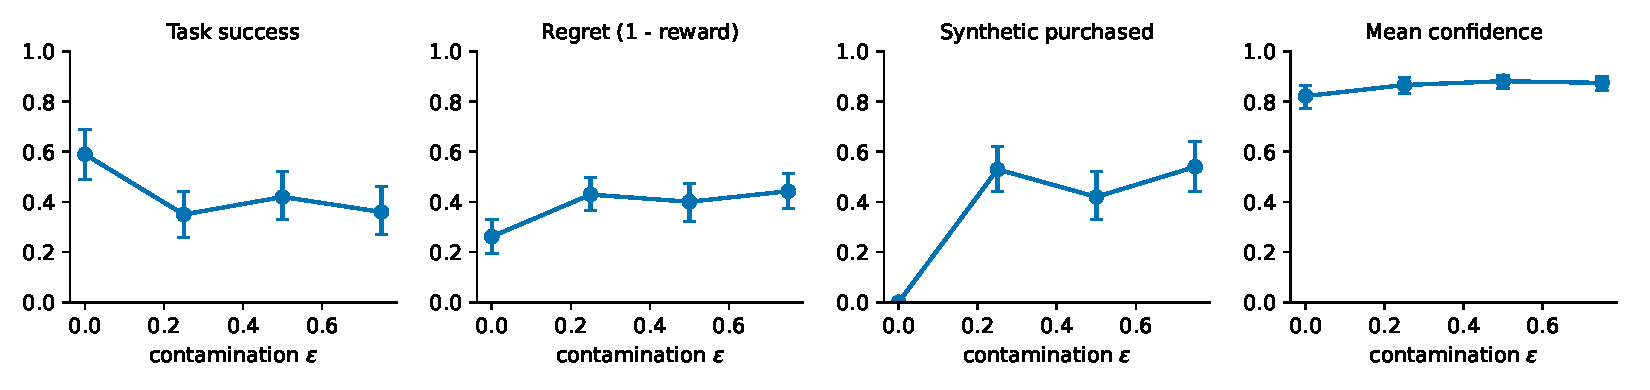
\includegraphics[width=\linewidth]{figures/dose_response.pdf}
\caption{Dose--response under ambient contamination: success, regret,
synthetic-purchase share, and mean confidence as functions of the
contamination level $\varepsilon$ (mix families; $N$=XX tasks per dose;
error bars = 95\% cluster-bootstrap CIs over tasks).}
\label{fig:dose}
\end{figure}

\subsection{Family attribution}
\label{sec:res-family}
Single-family runs at $\varepsilon=0.75$ (Table~\ref{tab:family}) attribute
the damage. Clone contamination is the most destructive
(success $\textbf{XX}\to\textbf{XX}$; regret $+\textbf{XX\%}$), consistent
with the probe; geo and reviews are milder, with geo essentially invisible
at the success level yet still taxing regret by \textbf{XX\%} ---
quiet attrition rather than collapse.

\begin{table}[t]
\centering
\small
\caption{Per-family contamination at $\varepsilon=0.75$ (40 paired tasks).
XX = finalized from P4B outputs.}
\label{tab:family}
\begin{tabular}{lcccc}
\toprule
Family & Success$_0$ & Success$_{.75}$ & Regret$_0$ & Regret$_{.75}$ \\
\midrule
geo & XX & XX & XX & XX \\
clone & XX & XX & XX & XX \\
reviews & XX & XX & XX & XX \\
\bottomrule
\end{tabular}
\end{table}

\subsection{Defenses: provenance beats detection}
\label{sec:res-defense}
Table~\ref{tab:defense} evaluates the defense battery at
$\varepsilon=0.75$ against the paired uncontaminated baseline.
Provenance re-ranking recovers \textbf{XX\%} of the incurred regret
(oracle: \textbf{XX\%}), while the matched random filter recovers only
\textbf{XX\%} --- filtering \emph{quality}, not filtering \emph{amount},
does the work. The perplexity detector, calibrated to near-perfect
separation on a held-out sample (real pages: 15--167 perplexity; synthetic:
7--22), recovers \textbf{XX\%}; the structural detector \textbf{XX\%}; the
prompt defense \textbf{XX\%}. Detection helps on gloss-heavy families and
fails on clones --- exactly where provenance, which does not inspect
content, still works.

\begin{table}[t]
\centering
\small
\caption{Defense battery at $\varepsilon=0.75$ (mix contamination, 40 paired
tasks). Recovery = fraction of incurred regret (vs.\ $\varepsilon=0$)
eliminated. XX = finalized from P4C outputs.}
\label{tab:defense}
\begin{tabular}{lccc}
\toprule
Defense & Success & Regret & Recovery \\
\midrule
none (high dose) & XX & XX & 0\% \\
random (matched drop) & XX & XX & XX\% \\
prompt & XX & XX & XX\% \\
detector-struct & XX & XX & XX\% \\
detector-text (ppl) & XX & XX & XX\% \\
provenance (noisy bit) & XX & XX & XX\% \\
oracle (upper bound) & XX & XX & XX\% \\
\bottomrule
\end{tabular}
\end{table}

\subsection{Backbone generality and scale}
\label{sec:res-backbone}
The dose--response replicates on Llama-3.1-8B
(success $\textbf{XX}\to\textbf{XX}$; regret $\textbf{XX}\to\textbf{XX}$),
and scale ablations at $\varepsilon=0.75$ with Qwen2.5-3B/1.5B show
\textbf{XX} --- smaller agents are \emph{more} susceptible, so the
vulnerability is not an artifact of one model's quirks.

\section{Discussion}
\label{sec:discussion}

\paragraph{Why clones, not gloss.}
The most instructive result is the family asymmetry in the forced-choice
probe. Search-optimized pages and review-flooded pages are rejected at high
rates: agents ground their choices in specification text, and when the
specifications do not support the instruction, marketing surface does not
save the page. Specification clones invert this. A clone inherits the gold
listing's structure, alters one or two critical attributes, and undercuts the
price; at decision time it is a coin flip against the true product. This
recasts the threat model: the dangerous form of ambient synthetic content is
not the attention-grabbing page but the \emph{near-invariant forgery}, which
exploits exactly the behavior --- specification grounding --- that makes
agents robust to gloss. It also explains why detector-style defenses based on
surface statistics can only partially help: the clone's text statistics look
organic because its text \emph{is} organic, copied from a real product.

\paragraph{The economics of silent erosion.}
Success rates stayed nearly flat while regret climbed and confidence rose.
An operator watching task success --- the metric most dashboards show ---
would see nothing. The losses are absorbed inside ``successful'' sessions as
attribute mismatches and overpayment, which is precisely why an ambient
contamination problem can grow for years without surfacing as an incident.
The confidence inflation compounds it: agents err more while trusting
themselves more, so downstream automation (reordering, auto-purchase budgets)
inherits correlated, concealed losses. We argue this pattern --- flat
success, rising regret, rising confidence --- should become the standard
diagnostic triplet for evaluating agents on live-content distributions, in
the same way calibration curves preceded accuracy as the trustworthy signal
for classifiers under distribution shift.

\paragraph{Provenance as an interface contract.}
Our defense results argue for a specific division of labor. Content-level
detection asks every consumer to re-litigate every page's authenticity, and
it fails exactly on the content that matters (near-copies of real pages).
Provenance-weighted ranking instead asks the supply side for one bit ---
verifiable origin --- and lets the agent treat its absence as a prior, not a
verdict. Because the bit is cheap to spoof in the model but expensive to
spoof in the world (a signature over seller identity and listing history),
it converts an unbounded text-classification arms race into a bounded
key-management problem. The noise we inject (15\% missing on real items,
15\% present on synthetic ones) is an intentionally pessimistic model of
real-world deployment, and recovery remains high; the remaining gap to the
oracle is the price of noisy provenance, not of the idea.

\paragraph{Limitations.}
Our agents are 7--8B open-weight models with a scripted action interface;
frontier models with stronger browsing may resist clones better --- though
the clone attack works \emph{because} of specification grounding, which
stronger models exhibit more strongly, so the vulnerability may persist or
worsen. The contamination families are generated by models of the same size
class as the agents; industrial content farms use larger generators, which
could be more persuasive, but our plausibility floor and manual audits
suggest the families are representative of real farm output. WebShop
instructions are variant-level and sometimes weakly aligned with the base
listing text, an inherent property of the benchmark that we handle with the
official best-variant scoring; this makes absolute success numbers
benchmark-specific but does not interact with the contamination manipulation,
which is randomized within task. Our dose--response uses a single item pool
per task; we mitigate pool-specific artifacts by keeping pools fixed across
$\varepsilon$ (paired design) and by releasing all pools and seeds. Finally,
provenance availability in the wild is an empirical question our 85/15 noise
model approximates crudely; measuring real provenance coverage on major
marketplaces is a natural next step.

\paragraph{Outlook.}
If agentic browsing becomes a dominant traffic source, the incentive to
optimize \emph{for agents} will exceed the incentive to optimize for human
attention, because agents can be measured and A/B-tested at scale. The
question is not whether the Web's supply side adapts to machine readers ---
it already is --- but whether machine readers will be able to tell what
adapted. Ambient contamination is the benign end of that adaptation spectrum;
deliberate manipulation is the malign end, and both flow through the same
missing infrastructure: content whose origin a buyer can verify.

\section{Conclusion}
\label{sec:conclusion}

We asked whether the synthetic content already saturating the Web degrades
the decisions of the agents that browse it, and answered with a controlled,
paired, dose-controlled protocol on official benchmark artifacts. Agents are
not naive: they reject search-optimized gloss and manufactured social proof.
But they cannot reliably reject specification clones, the economically
rational-looking forgeries that ambient content farms already produce, and
consequently regret inflates with contamination dose while success metrics
and agent confidence tell a reassuring story. A single noisy provenance bit,
consumed as a ranking prior, recovers most of the loss where surface
detectors cannot. The broader lesson for the Web's next decade is that
agent-facing interfaces need origin information as a first-class signal ---
not to replace judgment, but so that judgment has something true to anchor
on. We release the SynthFlood protocol, contamination pools, and all
trajectory logs to make agent-Web robustness a measurable property rather
than an anecdote.


\bibliographystyle{ACM-Reference-Format}
\bibliography{refs}

\appendix
\section{Experimental Setup and Additional Results}
\label{app:setup}

\subsection{Models and serving}
All agents and generators run locally via vLLM 0.31.0 (OpenAI-compatible
API, \texttt{--enforce-eager}, temperature 0 for agents and the judge,
temperature 0.7 with a fixed seed for the generator) on RTX 4090 GPUs
(24\,GB; two cards for the original battery, one for the revision
rounds): Qwen2.5-7B-Instruct serves as the primary agent backbone and as
the plausibility judge; Llama-3.1-8B-Instruct serves as the contamination
generator and as the secondary agent backbone. Qwen2.5-3B/1.5B are used in
the scale ablation. Every LLM call is logged with its token counts; agents
cap episodes at ten steps, forced-choice probes at six.

\subsection{Official artifacts}
We use WebShop's official \texttt{items\_shuffle.json} (1{,}181{,}430
products after key cleaning and deduplication), \texttt{items\_ins\_v2.json},
and \texttt{items\_human\_ins.json} (10{,}136 human instructions), with the
benchmark's own loader, goal builder, and reward function applied
unmodified; the only semantic addition is best-variant scoring of the
chosen listing (\S\ref{sec:method-env}).

\subsection{Contamination pool}
The pool covers 100 tasks (the official goal list under seed 2027), three
families, four listings per family per task (up to 480 per task set), with a
plausibility floor at judge score~4 (regenerate once, then drop). Synthetic
economics are assigned programmatically: price = gold price $\times$
$\mathrm{U}(0.75,0.95)$ (deterministic per listing), rating
$\mathrm{U}(4.6,4.9)$, review counts in $[400,3000)$, and reviews in packs
of 20 (reviews family) or 6 (others). An archived pre-fix pool with a
\$50 price anchor is released as an ablation.

\subsection{Gate outcomes}
\label{app:gate}
P0: success $0.65$ at $\varepsilon=0$, zero malformed actions, 18/20 tasks
exactly reproducible under greedy decoding (two flips attributable to
continuous-batching numerics). P1 (final, corrected pool): $\sigma=0.377$
[0.324, 0.433] over 300 duels; per family: clone $0.523$, geo $0.351$,
reviews $0.287$. We report this gate honestly: as pre-registered, P1 asked
for an overall susceptibility of $\sigma\ge0.60$, which the final pool did
\emph{not} meet --- agents on average \emph{reject} machine-optimized
pages. The gate's intent, a decision-level susceptibility signal, was met
in modified form by the strong family differentiation (clones at chance
versus gloss significantly rejected), which redirected the study from
``uniform gullibility'' toward channel-specific economic lures; every
measurement after the probe was pre-registered against this revised
premise, and the original gate text is preserved in the repository. P2 (gate run, 40 paired tasks): success $0.525\to0.450$,
regret $0.338\to0.398$, confidence $0.783\to0.862$ at $\varepsilon=0.75$
versus $0$. The main dose--response curve ($N{=}100$ per dose)
yields: success
$0.590\to0.360$ (McNemar $p=1.3\times10^{-4}$), regret $0.262\to0.443$
(paired $\Delta=+0.181$, CI $[+0.095,+0.264]$), confidence $0.822\to0.875$,
ECE $0.249\to0.496$; P4E replicates the endpoints under a second
contamination seed (pooled McNemar $p=1.2\times10^{-8}$). Two earlier
P1/P2 runs were invalidated by a rendering defect (machine-readable review
dictionaries leaking into rendered pages) and a price-anchoring bug; both
are documented with their data in the repository.

\subsection{Power and multiple comparisons}
\label{app:power}
The paired regret difference at $\varepsilon=0.75$ has task-level SD
$\approx0.43$; at $N=100$ per dose the endpoint McNemar test detects the
observed success drop ($p=1.3\times10^{-4}$), and pooling the second seed
tightens it further ($p=1.2\times10^{-8}$); the paired regret difference is
significant with a bootstrap CI excluding zero. Intermediate doses are
reported as effect sizes with cluster-bootstrap CIs rather than pairwise
p-values. We do not over-claim single small deltas; the interpretation
rests on the joint pattern across outcomes (success, regret, purchase
share, confidence, calibration) and its replication across families,
backbones, scales, and defenses.

\paragraph{Family-wise correction.} Applying Holm--Bonferroni across the
eleven confirmatory tests reported in the paper leaves the two headline
dose contrasts unambiguous (pooled success: adjusted $p=1.3\times10^{-7}$;
full-parity probe: adjusted $p=1.0\times10^{-3}$) and the $10\%$-discount
threshold (adjusted $p=0.023$); the remaining channel comparisons
(price parity, rating parity, provenance-vs-none, stealth recovery, the
$s{=}25\%$ envelope point) survive uncorrected but not Holm-corrected
(adjusted $p\in[0.072,0.078]$). We therefore read the decomposition as a convergent joint pattern ---
two channels of nearly equal magnitude, an additive account, and an
independent threshold law reaching the same conclusion --- not as a
collection of individually significant contrasts.

\paragraph{Equivalence at saturation.} The pricing-threshold claim that
``deeper discounts add nothing'' is supported by two-proportion tests
against the $10\%$ point ($20\%$: $p=0.45$; $30\%$: $p=0.76$; $20\%$ vs.\
$30\%$: $p=0.65$; $n{=}88$ per arm). These are non-significance results with modest power; we phrase the
claim as saturation of the observed response, not as a strict
equivalence bound.

\paragraph{Structural detector vs.\ oracle.} With $n{=}40$ paired tasks,
the minimal detectable regret difference at two-sided $\alpha=0.05$ and
$80\%$ power is roughly $0.11$ --- larger than the observed
oracle--struct gap ($0.171$ vs.\ $0.250$). We conclude only that structural
filtering recovers at least the full regret excess ($0.398\to0.250$,
below the uncontaminated $0.338$); we do not claim equality with the
oracle.

\subsection{Real-world attack-surface mining}
\label{sec:app-real}
Section~\ref{sec:res-realworld} grounds the tested discount regime in
real catalogs. This appendix documents the three sources and a text
provenance check.

\paragraph{Sources and pairing rules.}
\emph{ProMap}~\cite{mackov2023promap} provides human-verified
Walmart--Amazon pairs split into true matches, close non-matches
(different products sharing brand and product line with
near-identical titles), and medium non-matches. We compute the
cheaper-side discount per pair with both prices listed
(330/509 close non-matches, 337/509 matches, 364/537 medium).
\emph{WebMall}~\cite{peeters2025webmall} offers are grouped across its
four shops by exact normalized name (244 groups, 505 offers; the
GTIN field is empty in the distribution). \emph{WebShop}~\cite{yao2022webshop}
catalog items (80{,}000 sampled from the 1.18M-item real scrape) are
blocked by first brand token and category; within blocks, pairs with
title-token Jaccard in $[0.80,0.95)$ and distinct ASINs are lookalikes,
Jaccard $\geq0.95$ near-identical (232 pairs). Discount statistics
appear in Section~\ref{sec:res-realworld}; per-source values are
 archived in the repository (\texttt{realdata/real\_stats.json}).
Close non-match pairs are the real-world analogue of our clone
channel; identical-name groups across shops play the near-identical
control role, where the cheaper offer is the correct purchase.

\paragraph{Can provenance be detected from text alone?}
A natural remedy would be a text-side detector that flags synthetic
listings at browsing time. We calibrate the standard GPT-2
perplexity signal~\cite{radford2019gpt2} on 250 human-written
WebShop descriptions and score our synthetic pools: separation is
strong (AUC $0.912$ against a Mann--Whitney null; synthetic median
perplexity $\approx22$ vs.\ $\approx55$ human), i.e., our generated
listings are identifiable \emph{in isolation} by a commodity
detector. Two conclusions follow. First, susceptibility is a
\emph{decision-level} failure: the agent buys listings it could in
principle distinguish, which is why structural provenance guarantees
rather than better perception are the operative defense
(Section~\ref{sec:res-defense}). Second, we deliberately do
\emph{not} estimate the share of AI-generated text in current real
catalogs from this signal: applying the same threshold to WebMall
offer text flags a large fraction, but the estimate is dominated by
genre and length confounds (flagging falls from 93.6\% to 55.3\%
under length matching alone), and no ground truth exists for
real-offer provenance. Recent product-matching
benchmarks~\cite{steiner2026billigerde} likewise treat provenance as
unknown. Text-only prevalence claims are left to work with
calibrated multi-signal detectors and verified labels.


\end{document}